
\begin{frame}
  \frametitle{Ground truth}
  
  \begin{itemize}
\item ``a golden standard to which the learning algorithm needs to adapt'' -- James Kobielus
\end{itemize}
  
  
\end{frame}


\begin{frame}
  \frametitle{Intuition}  

  \begin{figure}[tbph]
    \centering
    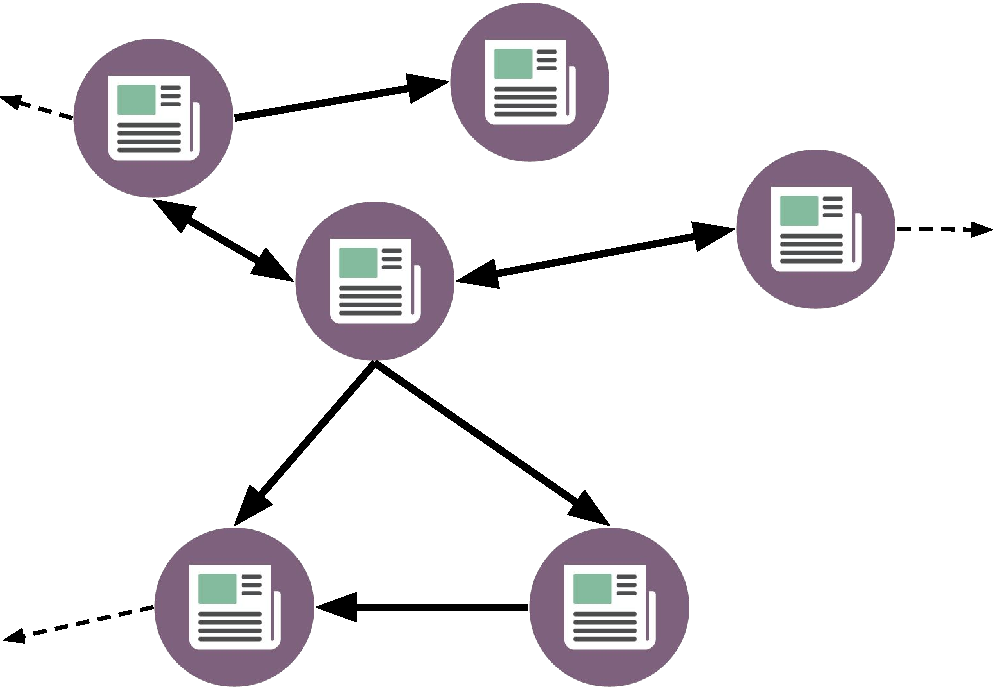
\includegraphics[width=0.5\linewidth]{images/wiki_gt_graph}
  \end{figure}
  
    \begin{itemize}
   \item Subgraph of Wikipedias article network
   \item Node: Article
   \item Edge: Hyperlink
   \begin{itemize}
  \item Weights are click frequencies
\end{itemize}
 
\end{itemize}
  
\end{frame}


\begin{frame}
  \frametitle{Prominent articles}
  
  Idea: Select articles that are good ``hubs'' and create a subgraph including all of their edges (hyperlinks).
  
    \begin{block}{Data in focus}
      \begin{itemize}
      \item 1000 \textit{prominent} articles
      \item 283k hyperlinks
      \item 144k unique \textit{prominent-linked} articles
	\end{itemize}
  \end{block}
  
\end{frame}


\begin{frame}
  \frametitle{Data in focus}
  
    \begin{figure}[tbph]
    \centering
    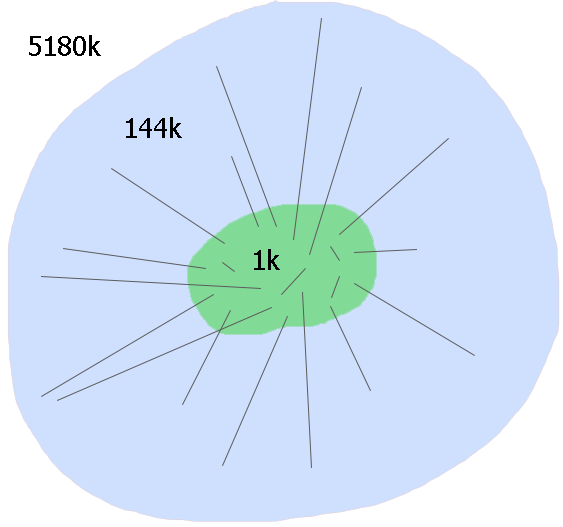
\includegraphics[width=0.5\linewidth]{images/potato}
  \end{figure}
  
\end{frame}


\begin{frame}
  \frametitle{Building ground truth file}
  
    \begin{figure}[tbph]
    \centering
    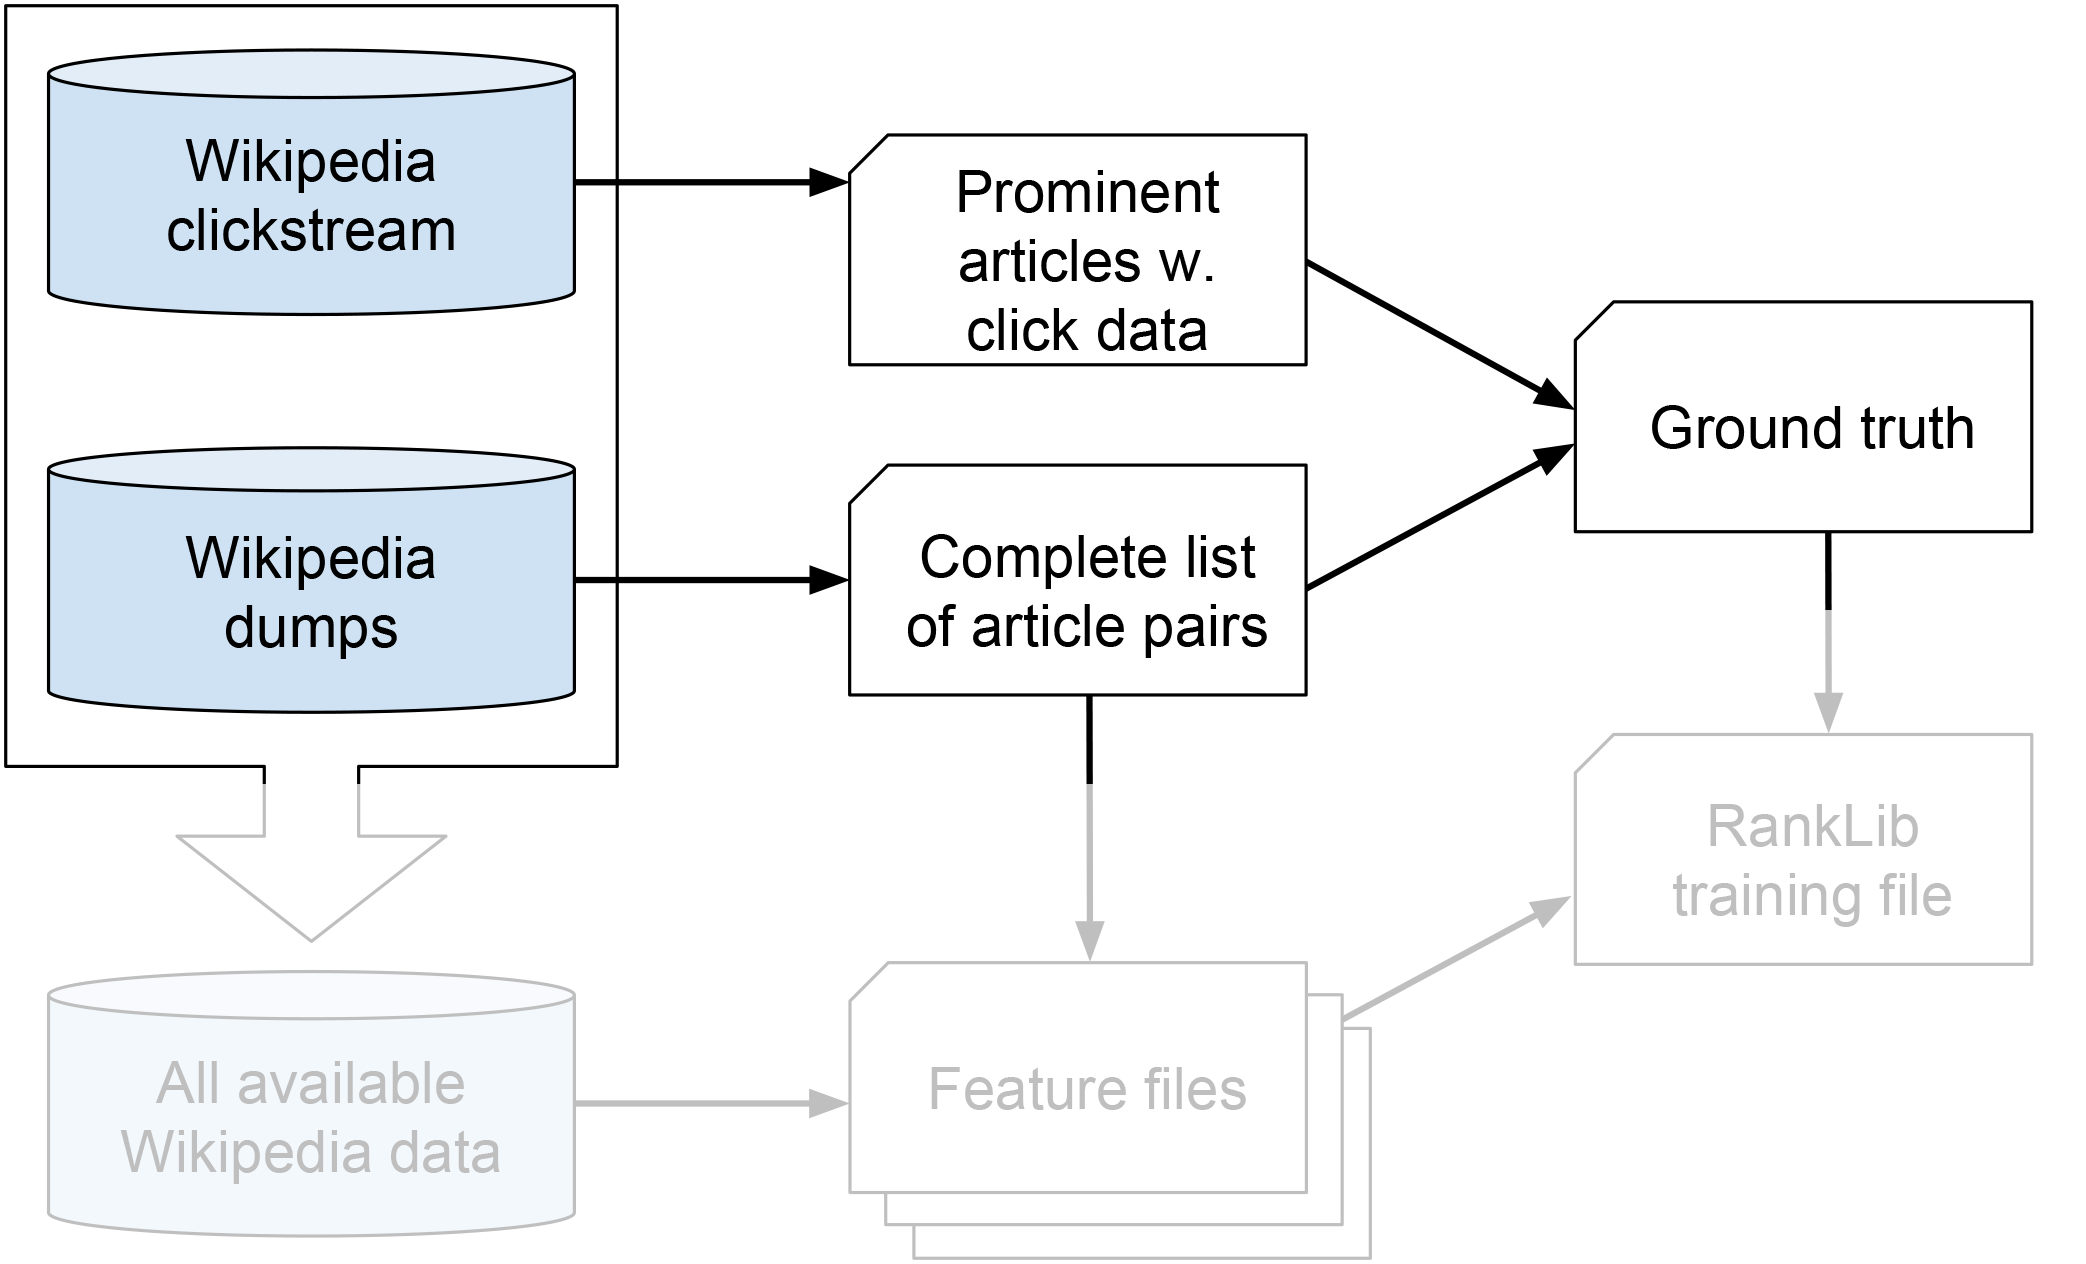
\includegraphics[width=0.9\linewidth]{images/process_gtfocus}
  \end{figure}
  
\end{frame}

\begin{frame}
  \frametitle{Example ground truth file}
  
  \begin{exampleblock}{Example of file content}	
  \begin{figure}[tbph]
    \centering
    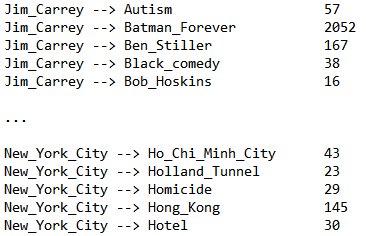
\includegraphics[width=0.7\linewidth]{images/GT_EXAMPLE}
  \end{figure}
  \end{exampleblock}

   
  
\end{frame}

\begin{frame}
  \frametitle{Building RankLib file}
  
      \begin{figure}[tbph]
    \centering
    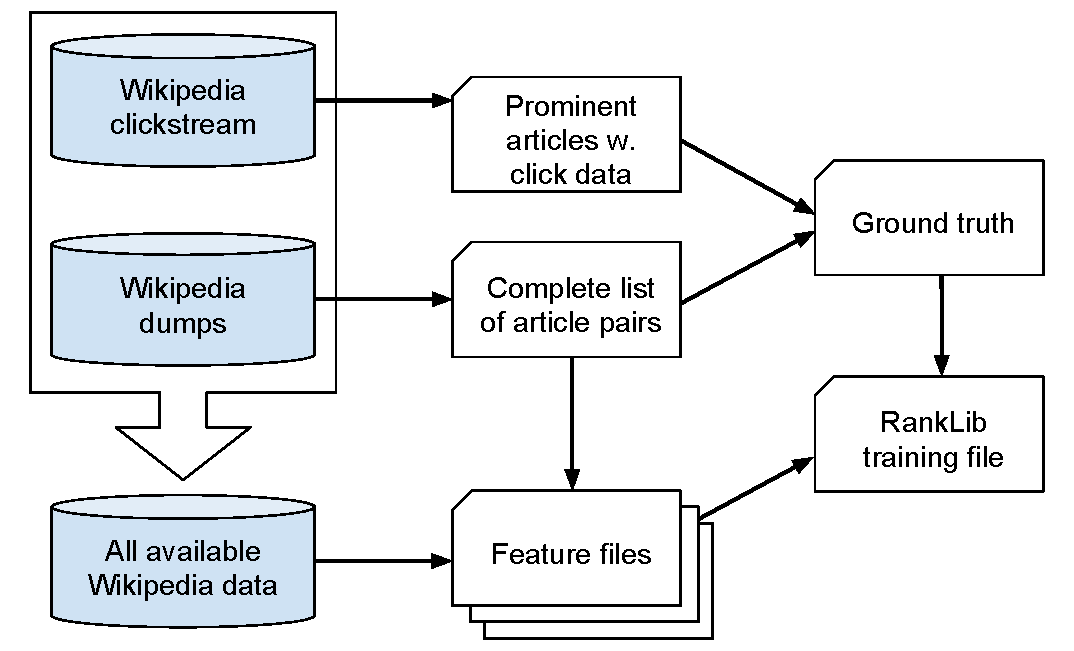
\includegraphics[width=0.9\linewidth]{images/process_small}
  \end{figure}
  
\end{frame}

\begin{frame}
  \frametitle{Example RankLib file}
  

  
    \begin{exampleblock}{Example of file content}	
   \begin{figure}[tbph]
    \centering
    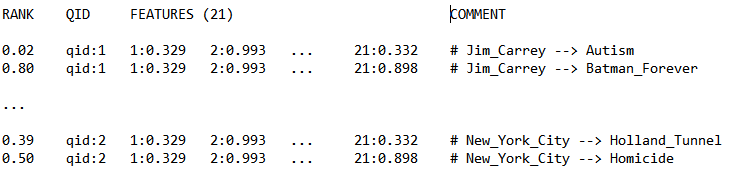
\includegraphics[width=1\linewidth]{images/ranklib_ex}
  \end{figure}
  \end{exampleblock}
  
\end{frame}

\begin{frame}
  \frametitle{Experimental setup}
  
  
   \begin{figure}[tbph]
    \centering
    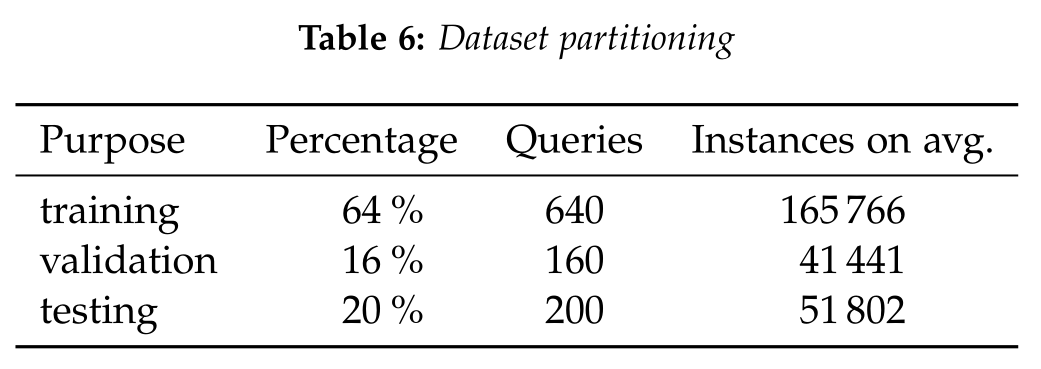
\includegraphics[width=0.7\linewidth]{images/expset}
  \end{figure}
  
  \centerline{5-fold cross-validation test}
  
  
\end{frame}

\begin{frame}
  \frametitle{Data complexity and difficulties}
  
  \begin{itemize}
\item Data processing in Python, R and Shell
\item Linux server for time consuming scripts
\item Well-structured (and defined) processing steps
\item Focus on low memory usage
\end{itemize}
  
  
\end{frame}

% slide 11: introducing ground truth
% slide 12: selection and extraction of prominent articles
% slide 13: constructing ground truth file w. figure 3
% slide 14: constructing rankLib file
% slide 14.5: table 6, experimental setup for supervised learning
% slide 14.7: difficulties and solutions for working with the wikipedia data